\documentclass[]{RRLPoster}
    \title{\parbox{\linewidth}{\centering Put Your Title Here}}
    \author{Benjamin Franklin, Thomas Jefferson}
    \date{\today}
    \institute{University of Pennsylvania}
    
    % These are for customizing the way that TikZ draws things, These aren't in the 
    % class to allow authors to change this 
    \usepackage{pgfplots}
    \pgfplotsset{compat=1.13}
    \usetikzlibrary{shapes,arrows,fit,positioning,patterns}
    \tikzstyle{block} = [rectangle, draw=colorTwo, very thick, fill=colorOne, 
    text centered, rounded corners, minimum height=2em, text=white]
    \tikzstyle{line} = [draw=colorTwo, latex'-latex', line width=1mm]
    \tikzstyle{mycloud} = [cloud, draw,cloud puffs=10,cloud puff arc=120, aspect=2, inner ysep=.2em]
    \usepackage[inline]{enumitem}
\begin{document}

\maketitle

\block{}{\centering \Large  
You can place a headline or abstract here, or delete this block. 
}

\begin{columns}
    \column{0.4}
    \block{Need}{
    \begin{itemize}
        \item This class is based off of tikz poster
        \item The idea is that you make columns to organize your poster
        \item You can nest columns
        \item You can change the number of columns part of the way down the page
    \end{itemize}
    }
    \block{System}{
    \begin{tikzfigure}
        
        \includegraphics[height=30cm]{images/naovgo.jpg}
        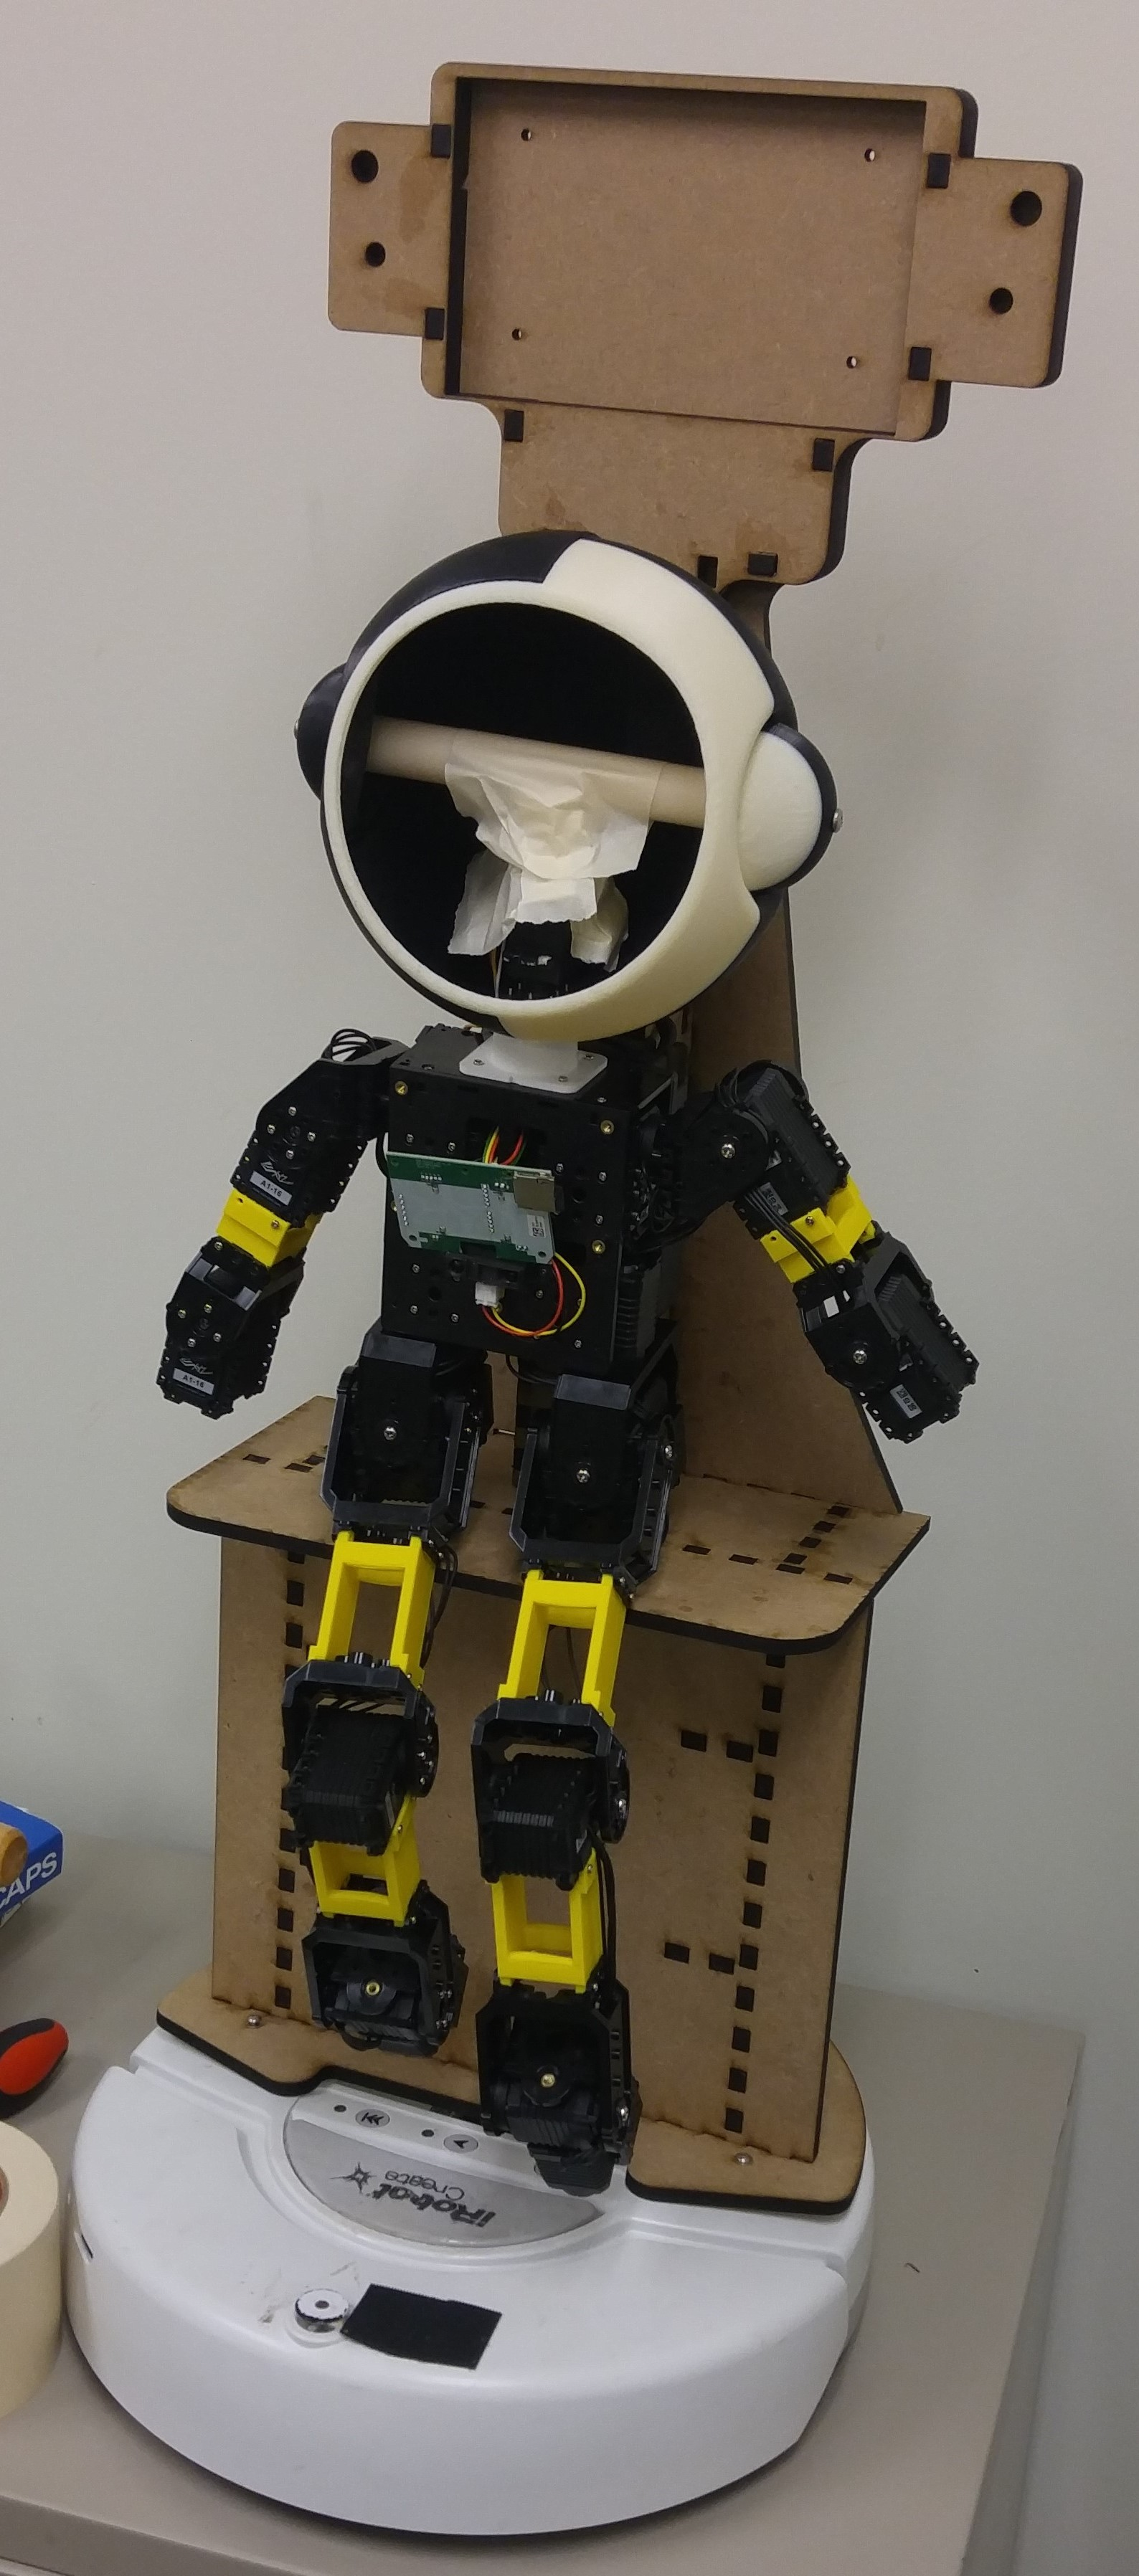
\includegraphics[height=30cm]{images/flo_head.jpg}
    \end{tikzfigure}
    You can include figures as show here
    \vspace{19pt}
    }
    \column{0.6}
    \block{A flowchart from visio}{
    \begin{tikzfigure}
        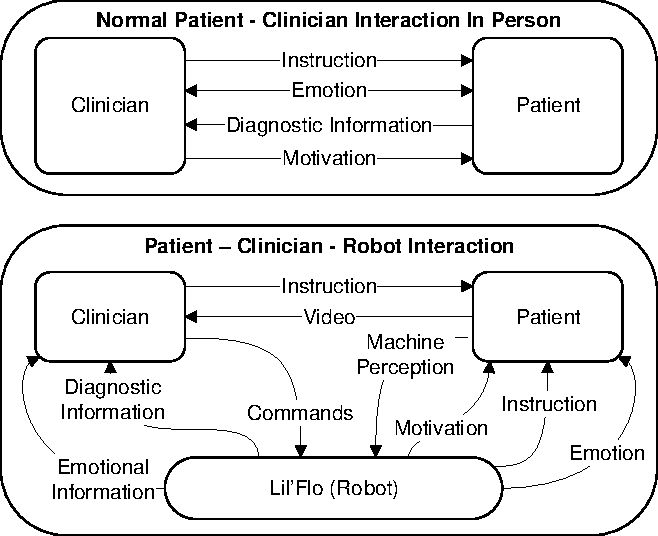
\includegraphics[width=30cm]{images/interaction.pdf}
    \end{tikzfigure}
    here is a flowchart from visio, it should be remade using tikz
    }
    \block{Some of the critical code}{
    \begin{itemize}
        \item You can change to have a landscape poster by changing the 
        top line to say: \texttt{\textbackslash documentclass[landscape]\{RRLPoster\}}
        \item You encase each set of columns by a \texttt{\textbackslash
        start{columns} and \textbackslash end{columns}}
        \item You then enter the columns (left to right) with a \texttt{
        \textbackslash column{<percent width you want>}}
        \item You then create a block with a call to \texttt{\textbackslash
        block{<block title>}{block contents}}
        \item You can find out more from the tikz poster sharelatex docs:\\
        https://www.sharelatex.com/learn/Posters\#Tikzposter
        \item You can also take a look at the tikz poster manual:\\
        http://mirror.hmc.edu/ctan/graphics/pgf/contrib/tikzposter/tikzposter.pdf)
    \end{itemize}
    }
\end{columns}

\begin{columns}
    \column{0.3}
    \block{taskse}{
    Here is a tikz based flowchart, kinda cool. 
    \centering
    \begin{tikzpicture}[node distance = .2cm and -.5cm, auto]
        % Place nodes
        \node [block] (server) {Server};
        \node [block, above left=of server] (user1) {User 1};
        \node [block, below left= of server] (user2) {User 2};
        \node [block, above right= of server] (robot1tm) {Task Manager};
        \node [block, below right =of server] (robot2tm) {Task Manager};
        \node [block,  above right= of robot1tm] (robot1controller2) {Ability 2 Controller}; 
        \node [block, above = of robot1controller2] (robot1controller1) {Ability 1 Controller}; 
        \node [block, below right= of robot2tm] (robot2controller1) {Ability 1 Controller}; 
        \node [block, below= of robot2controller1] (robot2controller2) {Ability 3 Controller}; 
        \node[draw=red,label=north:Robot 1, fit=(robot1tm) (robot1controller1)](robot1) {};
        \node[draw=red,label=south:Robot 2, fit=(robot2tm) (robot2controller2)](robot2) {};
        
        \path[line] (server.west) to [out=180, in=-90] (user1.south);
        \path[line] (server.west) to [out=180, in=90] (user2.north);
        
        \path[line] (server.north) to [out=90, in=180] (robot1tm.west);
        \path[line] (server.south) to [out=-90, in=180] (robot2tm.west);
        
        \path[line] (robot1tm.north) to [out=90, in=180] (robot1controller2.west);
        \path[line] (robot1tm.north) to [out=90, in=180] (robot1controller1.west);
        
        \path[line] (robot2tm.south) to [out=-90, in=180] (robot2controller2.west);
        \path[line] (robot2tm.south) to [out=-90, in=180] (robot2controller1.west);
        
    \end{tikzpicture}
    }
    \block{Paper Size}{You can set the paper size by passing an argument
    into the class call: \texttt{\textbackslash documentclass[<-here->]{RRLPoster}} 
        Your options are:
        \begin{itemize*}
            \item a0paper
            \item a1paper
            \item sz30x40
            \item sz40x30
        \end{itemize*}}
    \column{0.4}
    \block{A Table}{
    It is important for style that tables not have any vertical lines, as 
    seen here. You can find plenty of style guides on how to make good tables.
    \begin{center}
        \begin{tabular}{@{}lccccccc@{}}
            \toprule
            &\multicolumn{2}{c}{Inpatient/Outpatient}& 
            \phantom{a}& \multicolumn{2}{c}{Senior Day Care}& \phantom{a}\\
            \cmidrule{2-3} \cmidrule{5-6}
            & Average & Std. Error && Average & Std. Error && P-Value\\
            \midrule
            Intelligent?   & 2.98 & 0.17 && 3.55 & 0.18 && 0.03\\
            Helpful?       & 3.52 & 0.15 && 3.65 & 0.23 && 0.64\\
            Useful?        & 3.50 & 0.15 && 3.79 & 0.17 && 0.39\\ 
            Social?        & 3.02 & 0.14 && 3.32 & 0.25 && 0.31\\
            Communication? & 3.36 & 0.15 && 3.89 & 0.19 && 0.01\\
            \bottomrule
        \end{tabular}
    \end{center}
    }

    \block{A note on spacing}{
        Spacing in the vertical direction can be fixed by inserting more vspace. \\
        
        To see an example of what a really nice poster can look like, take a look
        at this:
        https://www.sharelatex.com/templates/other/fancy-tikz-poster
    }
    
    \column{0.3}
    \block{A pgf plot}{
\begin{tikzpicture}
\begin{axis}[
% title = {Optimization based upon co-occurences},
width=7in,
% height=5in,
bar width=.3in,
ymin=1,
ymax=5,
xtick={1,...,5},
xticklabels={%
Intelligent?  ,
Helpful?      ,
Useful?       ,
Social?       ,
Communication?},
grid=major,
xticklabel style={rotate=45,anchor=north east, align=right},
ylabel=Ratings (1-5),
ylabel near ticks,
legend style={at={(1.05,1.05)},anchor=north east},
ybar
]

\addplot[
fill=colorOne,
postaction={
pattern=crosshatch dots,
pattern color=white
},
draw=black,
point meta=y,
every node near coord/.style={inner ysep=5pt},
error bars/.cd,
y dir=both,
y explicit,
error bar style={line width=3pt}
] 
table [y error=error,row sep=crcr] {
x   y           error\\    
1   2.98        0.17\\  
2   3.52        0.15\\ 
3   3.50        0.15\\  
4   3.02        0.14\\  
5   3.36        0.15\\   
};

\addplot[
fill=colorTwo,
draw=black,
point meta=y,
every node near coord/.style={inner ysep=5pt},
error bars/.cd,
y dir=both,
y explicit,
error bar style={line width=3pt}
] 
table [y error=error,row sep=crcr] {
x   y           error\\  
1   3.55        0.18\\  
2   3.65        0.23\\ 
3   3.79        0.17\\  
4   3.32        0.25\\  
5   3.89        0.19\\  
};
\legend{In/Outpatient, Senior Day Care}
\end{axis}
\end{tikzpicture}
    }
\end{columns}

\makelogos
\end{document}
